\documentclass[crop,tikz,10pt]{standalone}

\usepackage{tikz-qtree}
\usetikzlibrary{calc}
\usetikzlibrary{arrows.meta}
\usetikzlibrary{decorations.text}
\usetikzlibrary{backgrounds}

\definecolor{bg1}{RGB}{244,231,195}
\definecolor{bg2}{RGB}{234,204,161}
\definecolor{l1}{RGB}{209,148,106}

\begin{document}

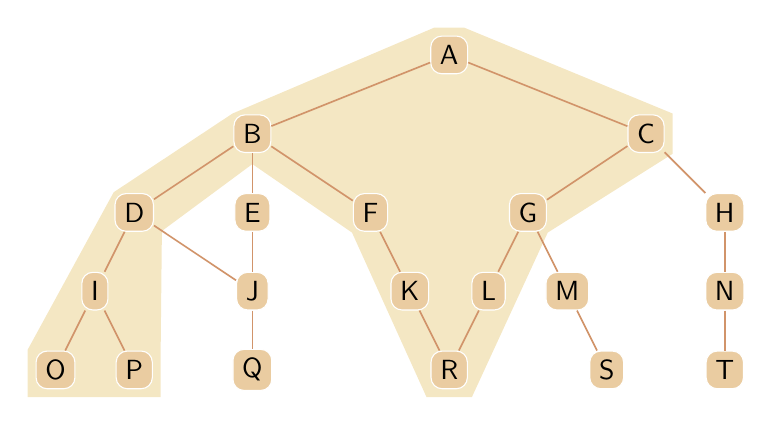
\begin{tikzpicture}[
    font=\sffamily,
    l/.style={
        line width=0.6pt,
        color=l1
    },
    e/.style={
        rounded corners,
        fill=bg2, draw=white, line width=0.4pt
    },
    ic/.style={font={\tiny},yshift=4pt,xshift=-4pt}
]

    \node [e] (A) at ( 0.5,  0) {A};
    \node [e] (B) at (-2  , -1) {B};
    \node [e] (C) at ( 3  , -1) {C};
    \node [e] (D) at (-3.5, -2) {D};
    \node [e] (E) at (-2  , -2) {E};
    \node [e] (F) at (-0.5, -2) {F};
    \node [e] (G) at ( 1.5, -2) {G};
    \node [e] (H) at ( 4  , -2) {H};
    \node [e] (I) at (-4  , -3) {I};
    \node [e] (J) at (-2  , -3) {J};
    \node [e] (K) at ( 0  , -3) {K};
    \node [e] (L) at ( 1  , -3) {L};
    \node [e] (M) at ( 2  , -3) {M};
    \node [e] (N) at ( 4  , -3) {N};
    \node [e] (O) at (-4.5, -4) {O};
    \node [e] (P) at (-3.5, -4) {P};
    \node [e] (Q) at (-2  , -4) {Q};
    \node [e] (R) at ( 0.5, -4) {R};
    \node [e] (S) at ( 2.5, -4) {S};
    \node [e] (T) at ( 4  , -4) {T};
    
    \draw (A) edge [l] (B);
    \draw (A) edge [l] (C);
    \draw (B) edge [l] (D);
    \draw (B) edge [l] (E);
    \draw (B) edge [l] (F);
    \draw (C) edge [l] (G);
    \draw (C) edge [l] (H);
    \draw (D) edge [l] (I);
    \draw (D) edge [l] (J);
    \draw (E) edge [l] (J);
    \draw (F) edge [l] (K);
    \draw (G) edge [l] (L);
    \draw (G) edge [l] (M);
    \draw (H) edge [l] (N);
    \draw (I) edge [l] (O);
    \draw (I) edge [l] (P);
    \draw (J) edge [l] (Q);
    \draw (K) edge [l] (R);
    \draw (L) edge [l] (R);
    \draw (M) edge [l] (S);
    \draw (N) edge [l] (T);
    
    \begin{scope}[on background layer]
        \fill [fill=bg1]
            ($(A.north)+(0mm, 1mm)$) --
            ($(A.north west)+(.5mm,1mm)$) --
            ($(B.north west)+(-.1mm,.1mm)$) --
            ($(D.north west)+(-.1mm,.1mm)$) --
            ($(O.north west)+(-1mm,.1mm)$) --
            ($(O.south west)+(-1mm,-1mm)$) --
            ($(P.south east)+(1mm,-1mm)$) --
            ($(P.north east)+(1mm,1mm)$) --
            ($(D.south east)+(1mm,.1mm)$) --
            ($(B.south)+(0mm,-1.4mm)$) --
            ($(F.south west)+(-.1mm,-.1mm)$) --
            ($(R.south west)+(-.5mm,-1mm)$) --
            ($(R.south east)+(.5mm,-1mm)$) --
            ($(G.south east)+(.1mm,-.1mm)$) --
            ($(C.south east)+(1mm,-.1mm)$) --
            ($(C.north east)+(1mm,.1mm)$) --
            ($(A.north east)+(-.5mm,1mm)$) -- cycle;
    \end{scope}
    
\end{tikzpicture}

\newpage

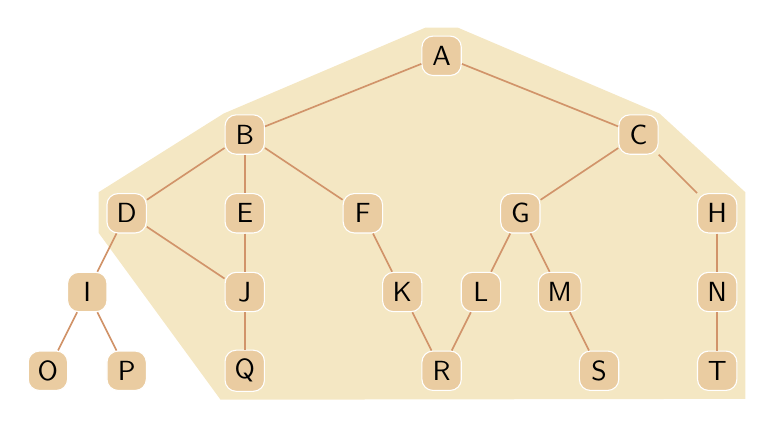
\begin{tikzpicture}[
    font=\sffamily,
    l/.style={
        line width=0.6pt,
        color=l1
    },
    e/.style={
        rounded corners, minimum width=0.5cm, minimum height=0.5cm,
        fill=bg2, draw=white, line width=0.4pt
    },
    ic/.style={font={\tiny},yshift=4pt,xshift=-4pt}
]

    \node [e] (A) at ( 0.5,  0) {A};
    \node [e] (B) at (-2  , -1) {B};
    \node [e] (C) at ( 3  , -1) {C};
    \node [e] (D) at (-3.5, -2) {D};
    \node [e] (E) at (-2  , -2) {E};
    \node [e] (F) at (-0.5, -2) {F};
    \node [e] (G) at ( 1.5, -2) {G};
    \node [e] (H) at ( 4  , -2) {H};
    \node [e] (I) at (-4  , -3) {I};
    \node [e] (J) at (-2  , -3) {J};
    \node [e] (K) at ( 0  , -3) {K};
    \node [e] (L) at ( 1  , -3) {L};
    \node [e] (M) at ( 2  , -3) {M};
    \node [e] (N) at ( 4  , -3) {N};
    \node [e] (O) at (-4.5, -4) {O};
    \node [e] (P) at (-3.5, -4) {P};
    \node [e] (Q) at (-2  , -4) {Q};
    \node [e] (R) at ( 0.5, -4) {R};
    \node [e] (S) at ( 2.5, -4) {S};
    \node [e] (T) at ( 4  , -4) {T};
    
    \draw (A) edge [l] (B);
    \draw (A) edge [l] (C);
    \draw (B) edge [l] (D);
    \draw (B) edge [l] (E);
    \draw (B) edge [l] (F);
    \draw (C) edge [l] (G);
    \draw (C) edge [l] (H);
    \draw (D) edge [l] (I);
    \draw (D) edge [l] (J);
    \draw (E) edge [l] (J);
    \draw (F) edge [l] (K);
    \draw (G) edge [l] (L);
    \draw (G) edge [l] (M);
    \draw (H) edge [l] (N);
    \draw (I) edge [l] (O);
    \draw (I) edge [l] (P);
    \draw (J) edge [l] (Q);
    \draw (K) edge [l] (R);
    \draw (L) edge [l] (R);
    \draw (M) edge [l] (S);
    \draw (N) edge [l] (T);
    
    \begin{scope}[on background layer]
        \fill [fill=bg1]
            ($(A.north)+(0mm, 1mm)$) --
            ($(A.north west)+(.5mm,1mm)$) --
            ($(B.north west)+(-.1mm,.1mm)$) --
            ($(D.north west)+(-1mm,.1mm)$) --
            ($(D.south west)+(-1mm,.1mm)$) --
            ($(Q.south west)+(-.5mm,-1mm)$) --
            ($(T.south east)+(1mm,-1mm)$) --
            ($(H.north east)+(1mm,.1mm)$) --
            ($(C.north east)+(.1mm,.1mm)$) --
            ($(A.north east)+(-.5mm,1mm)$) -- cycle;
    \end{scope}
    
\end{tikzpicture}

\end{document}
